\section{ОБЗОР ЛИТЕРАТУРЫ}
\label{sec:domain}
В части рассмотренных исследований решались смежные задачи, такие как жанровая классификация, идентификация музыкального трека, нахождение заимствований в музыкальном треке, распознавание  звуковых источников. Для решения данных задач использовались разные подходы к выделения информационных образов из музыкальных треков. Среди рассмотренных приложений также стоит отметить разнообразие подходов к выделению информационных признаков. В данной дипломной работе стоит задача найти такие характерные информационные образы, которые позволили на основе их делать рекомендацию
\subsection{Обзор методов выделения фрагментов из музыкальных произведений}
\label{sub:domain:overview_framing}
В работе\cite{src1}  информационные признаки, которые будут рассмотрены в следующем подразделе,  рассчитываются по фрагментам музыкального трека в 1 секунду, состоящему из 40 непересекающихся окон в  25 миллисекунд.  Для классификации используется 30 фрагментов. Полная сборка аудиоданных используемая в данной работе  состоит из 15 жанров * 50 файлов * 30 секунд = 22500 секунд (то есть 6,25 часов аудио). Каждый фрагмент  анализируется независимо. По каждому окну получают набор числовых? признаков. Их математическое ожидание и дисперсию используют в качестве признаков для фрагмента. В работе\cite{src2} используется такой же подход. Трёхсекундный фрагмент состоит из 1500 окон по 0,02 секунды. В отличии от работ\cite{src1} по автоматической жанровой классификации музыкального трека, в качестве признаков фрагмента используют  среднее значение, дисперсию, коэффициент асимметрии, коэффициент эксцесса информационных признаков окон. Эти четыре значения затем используются для измерения подобия. В работе\cite{src4}, где описывается принцип работы большинства аудиoидентификационных систем, используются фрагменты музыкального трека размером от 10 до 500 миллисекунд с перекрытием фрагментов от 50 до 90 процентов. В этой же работе описываются алгоритмы распознавания ремиксов. 

Каждый музыкальный трек проходит передискретизацию до частоты 44100 Гц. Затем берется  четырёхсекундный фрагмент.

Недостатками данных методов является потеря информации о структурах в музыкальном треке, которые не помещаются в один фрагмент.

\subsection{Обзор методов представления музыкального трека в спектрально-временном виде}
\label{sub:domain:overview_spectre}
В работе\cite{src3} решается задача идентификации(опознавания) музыкального трека, а также поиск заимствований в жанре музыки хип-хоп.  Для получения спектрограммы используется оконное преобразования Фурье с окном Хемминга и размером окна 64 миллисекунды. После получения спектрограммы используется только амплитудная составляющая с последующим логарифмированием и применением высокочастотного фильтра к спектральной кривой. Эти шаги предпринимаются для того, чтобы сделать спектрограмму менее зависимой от абсолютного уровня и грубой спектральной формы. Также в работе рассмотрено constant Q преобразование\cite{qtransform}. Выделение информационных признаков в  работе состоит из трёх стадий. Конечным результатом является коррелограмма. Первая стадия моделирует влияние  звуковой волны на базилярную мембрану ушной улитки с помощью полосового фильтра, который реализуется четырьмя каскадными секциями фильтра второго порядка, которые реализуют фильтр восьмого порядка с импульсной характеристикой <<gammatone>> c центральной частотой в 9,3 кГц. Вторая стадия моделирует движение  волосковых клеток. Так как клетки реагируют только на отклонение ресничек в одном направлении, и это вводит этап выпрямления в цепочке обработки сигналов. На низких частотах волосковые клетки имеют тенденцию срабатывать в определенной фазе сигнала - процесс, называемый блокировкой фазы. По мере того как частота входного сигнала увеличивается, блокировка фазы начинает заканчиваться примерно на 1,5 кГц и исчезает на 5 кГц, но при отсутствии блокировки тонкой структуры формы сигнала волосковые клетки фиксируются в амплитудной огибающей сигнала. Этот эффект моделируется посредством операции свертки с импульсным откликом фильтра типа <<приподнятого-косинуса>> \cite{raised_consinus} с T = 0,25 мс. Третья стадия это построение коррелограммы. Коррелограмма моделирует человеческое восприятия основного тона. Для этого используется автокорреляция.  Измерением средней энергии в зависимости от задержки можно определить базовый период сигнала. После FFT-преобразования считается оконная автокорреляция для частотной области. Полученный трёхмерный массив данных(время, частота, высота тона) используется для получения информационных признаков для классификации музыкальных инструментов. 
В работе симулируется человеческое восприятие. Механизмы распознавания в человеческом мозге гораздо лучше приспособлены к сложным акустическим средам, чем любой искусственный механизм (рисунок \ref{fig:domain:machine_limitation}). 

\begin{figure}[ht]
\centering
  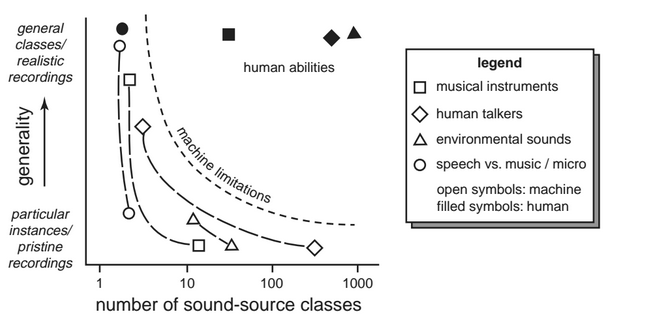
\includegraphics[scale=0.8]{machine_limitation.png}
  \caption{График показывающий ограничения искусственных механизмов распознавания}
  \label{fig:domain:machine_limitation}
\end{figure}

В работе для извлечения информационных образов о ритме используется вейвлет Добеши четвёртого порядка. 

\subsection{Обзор методов выделения информационных признаков}
\label{sub:domain:feature_extraction}
В работе различается два вида признаков: спектральные и временные. Временные признаки - это значения, которые вычисляются из значений самих аудиоданных. Спектральные -  на основе спектра полученного преобразованием Фурье. 

Временные признаки:
\begin{enumerate}[label=\arabic*.]
\item Количество переходов сигнала через ноль.
\begin{equation}\label{eq:zcr}
ZeroCrossignRate =  \frac{1}{N_S} \sum \limits_{i=0}^{N_S - 2} sgn(s_i)  \oplus sgn(s_{i+1})
\end{equation}  
где $ N_S $ - количество сэмплов в окне, $ sgn() $ - функция которая возвращает 1 при положительном значении аргумента, и 0 при отрицательном.  $ s $ - вектор, содержащий данные сигнала для одного окна	
\item Автокорреляция первого порядка.
\begin{equation}\label{eq:autocorrelation}
FirstOrderAutocorrelation =  \frac{1}{N_S} \sum \limits_{i=0}^{N_S - 2} s_i  * s_{i+1}
\end{equation}  
где $ N_S $ - количество сэмплов в окне,  $ s $ - вектор, содержащий данные сигнала для одного окна.	
\item Энергия сигнала.
\begin{equation}\label{eq:energy}
Energy =  \frac{1}{N_S} \sum \limits_{i=0}^{N_S - 1} ( s_i )^2
\end{equation}  
где $ N_S $ - количество сэмплов в окне,  $ s $ - вектор, содержащий данные сигнала для одного окна.	
\end{enumerate}

Спектральные признаки:

\begin{enumerate}[label=\arabic*.]
\item Линейная регрессия спектра
\begin{equation}\label{eq:regression}
\beta = \frac{ N_B \sum\limits_{i=1}^{N_B} (a_i F_i) -  \sum\limits_{i=1}^{N_B} a_i  \sum\limits_{i=1}^{N_B} F_i}{N_B\sum\limits_{i=1}^{N_B} (F_i)^2 - \sum\limits_{i=1}^{N_B} (F_i)^2 }
\end{equation}
где $a$ - амплитуда,  $N_B$ - количество компонент разложения, а $F$ - частота соответствующей амплитуды $а$.

Это статистическое приближение использовано для нахождения наклона $(\beta)$ спектра, который является мерой отношения высокочастотной составляющей к низкочастотной составляющей звука и, следовательно, тембра. 
\item Среднее арифметическое взвешенное спектра.
\begin{equation}\label{eq:centroid}
SpectralCentroid = \frac{\sum \limits_{i=1}^{N_B} a_i F_i}{\sum \limits_{i=1}^{N_B} a_i}  
\end{equation}  
Психоакустически это показатель воспринимаемой <<яркости>> звука, обеспечивающий лучшую оценку <<яркого>> звука, нежели тональность.
\item Гладкость спектра, как мера спектральной огибающей.
\begin{equation}\label{eq:smooth}
SSmoothness = \sum \limits_{i=1}^{N_B} 20 \log a_i - \frac{20 \log a_{i-1} + 20 \log a_i + 20 \log a_{i+1}}{3} 
\end{equation}  
где $ a $ - амплитуда,  а $N_B$ - количество компонент разложения. 
Белый шум, спектр которого имеет энергию на всех частотах будет иметь гладкость 1. Синусоидальный сигнал имеет только один пик в спектре и гладкость спектра будет равняться 0. 
\item Дисперсия спектра относительно его среднего взвешенного.  Оркестровые треки будут иметь большее значение, в отличии от сольных или  монофонический треков. Вычисляется по следующей формуле:  
\begin{equation}\label{eq:spread}
SSpread = \sqrt{\frac{ \sum \limits_{i=1}^{N_B} a_i ( F_i - SpectralCentroid)^2 }{\sum \limits_{i=1}^{N_B} a_i}} 
\end{equation}  
где $a$ - амплитуда, $SpectralCentroid$ - центроида спектра,  $N_B$ - количество компонент разложения, а $F$ - частота соответствующей амплитуды $ а $.
\item Коэффициент асимметрии сигнала, является мерой того, насколько искажён спектр относительно  его среднего взвешенного.
\begin{equation}\label{eq:Dissymmetry}
SDissymmetry = \sqrt{\frac{ \sum \limits_{i=1}^{N_B} a_i ( F_i - SpectralCentroid)^3 }{\sum \limits_{i=1}^{N_B} a_i}} 
\end{equation}  
\end{enumerate}


В работе\cite{src1} исследованы алгоритмы автоматической жанровой классификации. Предложены набор признаков для представления <<музыкальных аспектов>> и ритмических структур аудиосигнала. 

Термин <<музыкальные аспекты>> используются для обозначения особенности музыки, связанные с текстурой, тембром и музыкальными инструментами. В работе используется 4 статистических информационных образов, представляющие собой мат. ожидания и СКО следующих числовых признаков:

\begin{enumerate}[label=\arabic*.]
\item Среднее арифметическое взвешенное спектра, как мера спектральной яркости (см. формулу \ref{eq:centroid}).
\item Энергетические спектральные окна по уровню 0,85.
\begin{equation}\label{eq:rolloff}
 \sum\limits_{i=1}^{Rolloff} a_i =  \sum\limits_{i=1}^{N_B} a_i
\end{equation}  
где $ a $ - амплитуда,  а $N_B$ - количество компонент разложения. 
\item Производная по частотам.
\begin{equation}\label{eq:flux}
Flux = \lVert a_i - a_p \rVert
\end{equation}  
где $a_i$ - амплитуда текущего окна, $a_p$ - амплитуда прошлого окна.
\item Количества переходов через ноль сигнала, как показатель зашумленности сигнала (см. формулу \ref{eq:zcr}).
\end{enumerate}

Дополнительно выделяется процент окон, чья спектральная энергия меньше чем средняя спектральная энергия по фрагменту.

Также выделяются ритмические признаки. Вычисление признаков для представления ритмической структуры музыки основано на вейвлет преобразовании с вейвлетом Добеши. К результату вейвлет преобразования применяется автокорреляционная функция. Фиксируется первые пять пиков автокорреляционной функции и их соответствующие периодичности в ударах в минуту рассчитываются и добавляются в <<ритмическую>> гистограмму (см. рисунок \ref{fig:domain:histogramm}). Этот процесс повторяется итерацией по сигналу и накоплением периодичности в гистограмме. 

\begin{figure}[ht]
\centering
  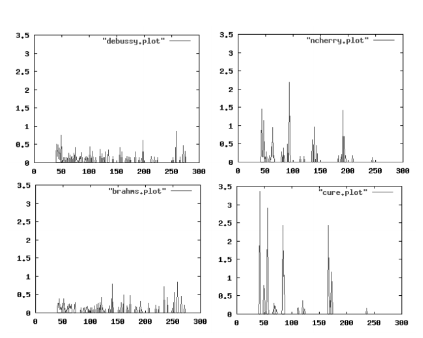
\includegraphics{histogramm.png}
  \caption{Гистограмма ритма. Cлева классическая музыка, справа поп-музыка}
  \label{fig:domain:histogramm}
\end{figure}

Пики гистограммы соответствуют различным периодичности звукового сигнала и используются в качестве основы для расчета признаков ритма. Используются следующие признаки, основанные на <<ритмической>> гистограмме :
\begin{enumerate}[label=\arabic*.]
\item Период - 0: Периодичность в ударах в минуту первого пика. 
\item Амплитуда - 0: Относительная амплитуда (деленная на сумму амплитуд) первого пика.
\item Отношение периодичности - 1: отношение периодичности второго пика к периодичности первого пика.
\item Амплитуда - 1: Относительная амплитуда второго пика.
\item Отношение периодичности - 2: отношения периодичности третьего пика к периодичности второго пика.
\item Амплитуда - 2: Относительная амплитуда третьего пика.
\item Отношение периодичности - 3: отношения периодичности четвёртого пика к периодичности третьего пика.
\item Амплитуда - 3: Относительная амплитуда третьего пика.
\end{enumerate}

8-мерный вектор признаков, используемый для представления ритмической структуры и силы, комбинируется с 9-мерным вектором музыкальной поверхности( 4 статистических информационных образа * 2 параметра), чтобы сформировать 17-мерный вектор признаков, который используется для автоматической классификации музыкального жанра.
В работе \cite{src2}  вводят меру спектральной плоскостности и коэффициент амплитуды.
\begin{equation}\label{eq:sfm}
SFM_k= \frac{[\prod S^2_k(f)]^{\frac{1}{N}} }{\frac{1}{N} \sum_f S^2_k(f)}	
\end{equation}
\begin{equation}\label{eq:scf}
SCF_k =  \frac{max_k S^2_K(k)}{\frac{1}{N} \sum_k S^2_K(k)}
\end{equation}
где $ S^2 $ - спектральная плотность мощности.

Чувственный эквивалент этих признаков можно охарактеризовать как шумоподобность и тоноподобие. Признаки с чувственным значением представляют характеристики звука, которые с большей вероятностью сохраняются в течении произведения и, следовательно, должны быть более надежными 

\subsection{Мел-кепстральные коэффициенты(MFCC)}
\label{sub:domain:overview_mffc}
Мел - психофизическая единица высоты звука, применяется
главным образом в музыкальной акустике. Количественная оценка звука по высоте основана на статистической обработке большого числа данных о субъективном восприятии высоты звуковых тонов. Звуковые колебания частотой 1000 Гц при эффективном звуковом давлении $2 * 10 ^{-3} $ Па (то есть при уровне громкости 40 фон), воздействующие спереди на наблюдателя с нормальным слухом, вызывают у него восприятие высоты звука, оцениваемое по определению в 1000 мел. Звук частоты 20 Гц при уровне громкости 40 фон обладает по определению нулевой высотой (0 мел). Зависимость нелинейна, особенно при низких частотах (для <<низких>> звуков). Преобразовать значение частоты звука (Гц) в значение высоты (мел) можно по формуле:
\begin{equation}\label{eq:mel}
m = 1127,01048 \ln(1 - \frac{f}{700})
\end{equation}

При обработке звука мел-частотный кепстр (MFC) представляет собой кратковременный спектр мощности звука, основанный на косинус - преобразовании Фурье на логарифмической спектральной мощности  на нелинейной мел-шкале частот.

Мел-кепстральные коэффициенты (MFCC) - это коэффициенты, которые в совокупности образуют MFC. Различие между кепстром и мел-кепстром в том, что в MFC полосы частот равномерно распределены по шкале мела, что приближается к восприятию слуховой системы человека более близко, чем линейные интервалы частот, используемые в нормальном кепстре.

MFCC обычно используются в качестве образов в системах распознавания речи, таких как системы, которые могут автоматически распознавать номера телефонов, произносимые в телефоне. MFCC также все чаще находят применение в приложениях поиска музыкальной информации, таких как классификация жанров\cite{mfcc2}, меры сходства звука\cite{mfcc1} и т. д.
\begin{figure}
\centering
  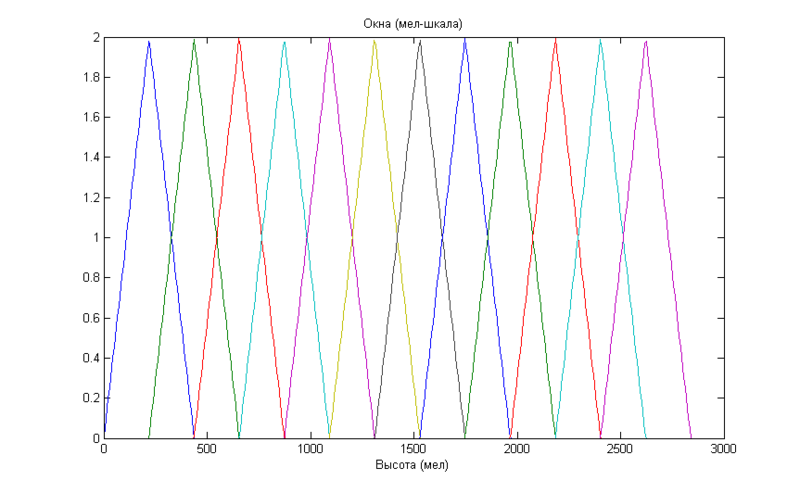
\includegraphics[scale=0.6]{mel_scale.png}
  \caption{Треугольные окна в мел-шкале}
  \label{fig:domain:mel_scale}
\end{figure}
\begin{figure}
\centering
  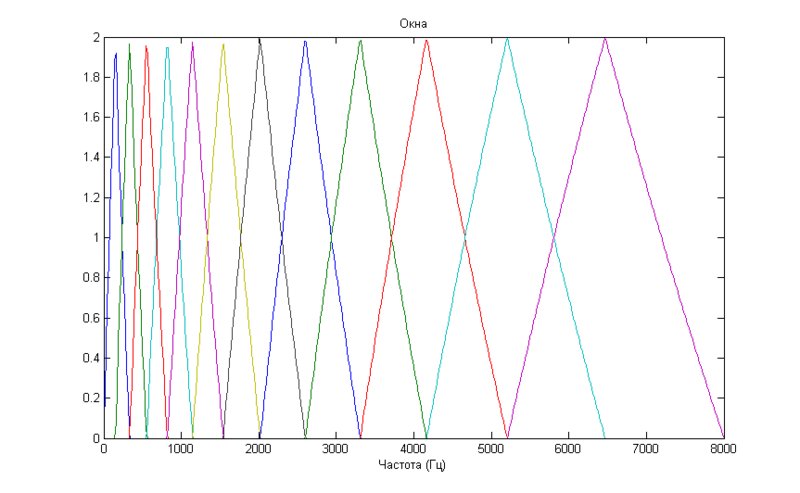
\includegraphics[scale=0.45]{freq_scale.png}
  \caption{треугольные окна в частотной шкале}
  \label{fig:domain:freq_scale}
\end{figure}


Для получения коэффициентов используют следующий алгоритм:
\begin{enumerate}[label=\arabic*.]
\item Используя преобразование Фурье получить спектр исходного сигнала.
\item Располагаем треугольные окна равномерно на мел-шкале (см. рисунок \ref{fig:domain:mel_scale}).
\item Переводим треугольные окна в частотную шкалу по формуле:
\begin{equation}\label{eq:flux}
f= 700(e^{\frac{m}{1127}} - 1)
\end{equation}  
\item Делаем свёртку спектра с каждым окном (см. рисунок \ref{fig:domain:freq_scale}) и берём логарифм спектра можности.
\item Полученные значения переводим во временную область дискретным косинусным преобразованием.
\item MFCC представляют собой амплитуды результирующего спектра.
\end{enumerate}



\subsection{Обзор аналогов}
\label{sub:domain:overview_analog}
\subsubsection {HOLO}

Данный проект - это приложение, которое по анализу музыкальной коллекции позволяет составлять плейлисты похожих на заданные образцы композиции, а также визуализировать полученные данные о музыкальной коллекции\cite{holo_blog}. Метод получение информационных признаков основан на преобразовании Фурье с последующим получением евклидового расстояния до набора готовых спектров, с последующим построением матрицы переходов. Спектры носят служебную функцию опорных значений, и их форма выбрана по принципу отличаться друг от друга как можно сильнее, как по громкости, так и по корреляции графика частот.
Формирование базы данных реализовано следующим образом:
\begin{enumerate}[label=\arabic*.]
\item Из файла извлекается фрагмент параметризуемой длины, начиная с 20\% общей длины.
\item Фрагмент нарезается на параметризуемое количество окон с параметризуемым процентом перекрытия.
\item Каждое окно подвергается преобразованию Фурье, сглаживанию и очистке.
\item Имея некоторый набор заранее подготовленных центроидов, оценивается расстояние каждого окна до каждого из этих центроидов.
\item На основе расстояния окно маркируется порядковым номером ближайшей центроиды.
\item Строится матрица переходов между номерами центроид(рисунок \ref{fig:domain:holo:matrix}).
\item Матрица переходов используется как вектор информационных признаков на основе которого происходит рекомендация.
\end{enumerate}
Также в приложении реализовано визуализация результатов сканирования локальной музыкальной библиотеки.

\begin{figure}
\centering
  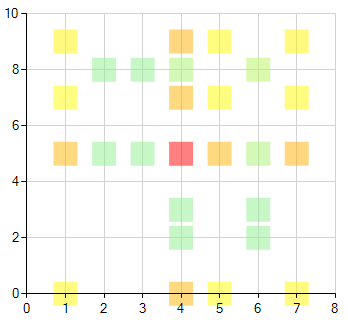
\includegraphics{HOLO_matrix.png}  
  \caption{Матрица переходов}
  \label{fig:domain:holo:matrix}
\end{figure}

Преимущества данного приложение:
\begin{itemize}
\item быстродействие;
\item иcпользует акустический анализ.
\end{itemize}
Минусы:
\begin{itemize}
\item нет взаимодействия с другими сервисами воспроизведения музыки;
\item используется только 20\% музыкального трека;
\item анализируются только MP3-файлы 44,1кГц 16 бит;
\end{itemize}

\subsubsection {Athena-NeuroPlay}
Данный проект  - это приложение, которое использует генетический алгоритм, который на основе оценки пользователя качества исходной выборки строит топологию нейронной сети прямого распространения с несколькими скрытыми слоями \cite{athena}.

Первый этап -  нормализация данных. Для инструментов выделяются необходимые частоты . Также принимается в расчёт и чувствительность слуха в зависимости от частоты.
Таким образом задача нормализации сводится к выделению некоторой информации о частотах, которая показывает:
\begin{itemize}
\item как часто в композиции звучит звук из данного диапазона частот;
\item как громко он звучал;
\item как долго он звучал;
\item для каждого определенного диапазона частот (нужно разбить весь <<слышимый>> спектр на определенное число диапазонов(см. рисунок \ref{fig:domain:athena:range} )).
\end{itemize}




Для выделения частотной насыщенности в треке на каждом временном интервале используется FFT. Временной интервал имеет размер 1024 сэмплов. На основе спектра получают следующие признаки: насыщенность звука определенными спектрами, частота возникновения различных спектров звука, его громкость, его длительность. Затем данные нормализуются.

\begin{figure}[h]
\centering
  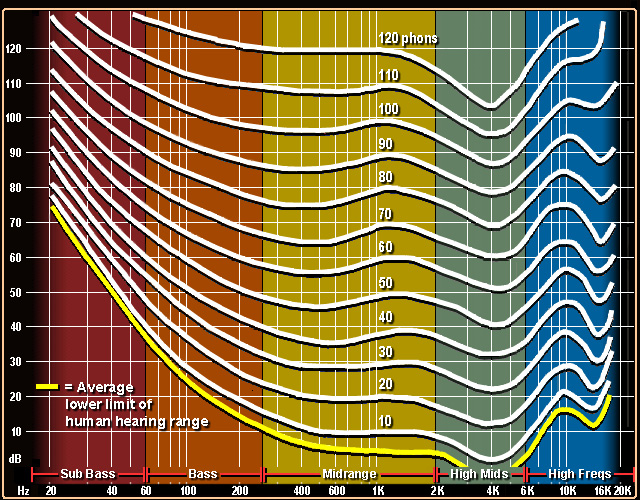
\includegraphics[scale=0.5]{range.jpg}  
  \caption{Диапазоны  частот}
  \label{fig:domain:athena:range}
\end{figure}

На втором этапе используется нейронная сеть прямого распространения с 1024 входными нейронами и 24*7 выходными, где каждый выходной нейрон показывает <<качество>> трека для того или иного времени суток.  В качестве исходной выборки используется плейлист, который делится на две части: обучающая и контрольная. Размер обучающей и контрольной выборке устанавливается пользователем. При прослушивании трека из обучающей выборке пользователь ставит оценку от 0 до 1, где 0 - <<плохой трек>>, а 1 - <<хороший>>. Оценка влияет на все оценки по времени суток, но больше на ту, в которое время было поставлена оценка.  После того как обучающая выборка промаркирована, идёт процесс обучения и настройки топологии нейронной сети. Топология нейронной сети  определяется генетическим алгоритмом. Для этого берётся стартовая конфигурация в 10 слоев, в каждом по 100 нейронов, которая обучается за 1000 эпох, после определятся качество ее обучения. Качество обучения - это суммарная оценка контролирующей и обобщающей способности нейронной сети. На следующем этапе создаётся 10 конфигураций, каждая из которых является <<мутантом>> исходной, то есть у нее изменена в случайную сторону либо количество слоев, либо количество нейронов на каждом или некоторых слоях. Далее идёт обучение каждой конфигурации тем же способом, что и исходную. Выбирается лучшая из них по обобщающей способности  и определяется как исходная. Данный процесс продолжаем до тех пор, пока не наступает такой момент, что мы не можем найти конфигурацию, которая обучается лучше чем исходная. Данную конфигурацию считаем лучшей, она оказалась способной лучше всех <<запомнить>> исходные данные и лучше всех предсказывает, то есть результат ее обучения наиболее качественный из возможных.





Из плюсов данного приложения стоит отметить:
\begin{itemize}
\item использует акустический анализ;
\item запускается локально на компьютере пользователя.
\end{itemize}

Из недостатков:
\begin{itemize}
\item время работы;
\item качество рекомендации.
\end{itemize}



\subsubsection {Pandora Radio}

Pandora (Пандора) - служба потокового воспроизведения музыки в Интернете, основанное на  системе <<Music Genome Project>> \cite{pandora_blog}. Пользователь медиапроигрывателя Pandora выбирает музыкального исполнителя, после чего система ищет похожие композиции, используя около 400 музыкальных характеристик такие как жанр, тип инструментов, тип вокала, темп, синкопа, тональность, гармония и т. д. Используя функции <<нравится>> или <<не нравится>>, слушатель может настроить <<радиостанцию>> по своему вкусу. В базе данных системы более миллиона композиций и более ста тысяч исполнителей\cite{tech_blog}. Зарегистрированный пользователь может создать в своём профиле до 100 различных <<радиостанций>>, транслирующих музыку в тех или иных жанрах. Медиапроигрыватель Pandora доступен пользователям с персональными компьютерами, смартфонами, планшетами с различными операционными системами.

Проект <<Music Genome Project>> - это набор более 450 атрибутов для описания песен и сложный математический алгоритм для их организации. Проект в настоящее время состоит из 5 суб-геномов : Pop / Rock, Hip-Hop / Electronica, Jazz, World Music и Classical. Песня представляется вектором, содержащим значения приблизительно для 450 <<генов>>. Каждый ген соответствует характеристике музыки, например, пол ведущего вокалиста, уровень искажения на электрогитаре, тип фонового вокала и так далее. Рок и поп-песни имеют 150 генов, рэп-песни имеют 350 генов, а джазовые песни - приблизительно 400. Другие жанры музыки, такие как мировая и классическая музыка, имеют 300-450 генов. Система зависит от достаточного количества генов для получения полезных результатов. Учитывая вектор одной или нескольких песен, список других подобных песен построен с использованием того, что компания называет своим <<алгоритмом сопоставления>> \cite{google_patent}. Атрибуты для каждой песни выставляются музыкантом в процессе, который занимает от 20 до 30 минут на песню\cite{interview}. Десять процентов песен анализируются более чем одним музыкантом, чтобы обеспечить соответствие внутренним стандартам и статистическую надежность.

Преимущества данного сервиса:
\begin{itemize}
\item большая база данных музыки;
\item имеются приложения для десктопов и мобильных платформ;
\item быстродействие;
\item взаимодействия с другими сервисами.
\end{itemize}

Из недостатков стоит отметить:
\begin{itemize}
\item cервис недоступен за пределами США, Австралии и Новой Зеландии;
\item требуется регистрация;
\item акустический анализ представлен не в чистом виде.
\end{itemize}



\subsection{Выбор информационных образов для жанровой классификации музыкальных произведений}
\label{sub:domain:feature_selection}
На основе анализа литературы были выбраны четыре типа информационных образов, которые будут извлекаться из музыкального трека:
\begin{itemize}
\item временной образ;
\item спетральный образ;
\item ритмический образ;
\item мел-кепстральный образ.
\end{itemize}

Временные образ (здесь и далее представления музыкального трека как набора отсчётов будет называться сигналом).

\begin{enumerate}[label=\arabic*.]
\item Энергия сигнала, как мера яркости и громкости мелодии (см. формулу \ref{eq:energy}).
\item Количество переходов сигнала, через ноль, как мера зашумлённости (см. формулу \ref{eq:zcr}).
\item Автокорреляция сигнала, как мера изменения резкости тембра (см. формулу \ref{eq:autocorrelation}.
\end{enumerate}

Спектральный образ.

\begin{enumerate}[label=\arabic*.]
\item Среднее арифметическое взвешенное спектра. С точки зрения восприятия, оно имеет робастную связь с впечатлением <<яркости>> звука (см. формулу \ref{eq:centroid}).
\item Линейная регрессия спектра, как мера отношения высокочастотной составляющей к низкочастотной составляющей звука и, следовательно, тембра (см. формулу \ref{eq:regression}).
\item Гладкость спектра, как мера гармоничности сигнала (см. формулу \ref{eq:smooth}).
\item Дисперсия спектра относительно среднего взвешенного. С точки зрения восприятия, определяет <<ширину>> тембра (см. формулу \ref{eq:spread}).
\item Коэффициент асимметрии, как мера того, насколько искажён спектр относительно среднего взвешенного спектра, и, следовательно наклон к высоким или низким частотам (см. формулу \ref{eq:Dissymmetry}).
\item Энтропия Винера или мера спектральной плоскостности. Определяет зашумлённость сигнала. Чем меньше значение, тем больше спектральной мощности сосредоточено в относительно небольшом числе полос (см. формулу \ref{eq:scf}).
\item Энергетическое спектральное окно по уровню 0,85, как мера спектральной формы (см. формулу \ref{eq:rolloff})
\item Коэффициент амплитуды (см. формулу \ref{eq:sfm}). 
\end{enumerate}

Ритмический образ.
Признаки считаются по коррелограмме.
\begin{enumerate}[label=\arabic*.]
\item Амплитуда первого пика.
\item Отношение частот первого пика к частоте второго пика.
\item Амплитуда второго пика.
\item Отношение частот второго пика к частоте третьего пика.
\item Амплитуда третьего пика.
\item Отношение частот третьего пика к частоте четвёртого пика.
\item Амплитуда четвёртого пика.
\item Частота первого пика.
\end{enumerate}

Мел-кепстральный образ представляет из себя 16 мел-кепстральных коэффициентов.
